\documentclass{article}
\linespread{1.6}
\usepackage{graphicx}
\usepackage[margin=1in]{geometry}
\usepackage{indentfirst}
\usepackage{enumerate}
\usepackage{color}

\definecolor{royalbluedark}{RGB}{55,95,145}
\definecolor{royalblue}{RGB}{80,130,190}

\begin{document}
\title{Project Testing and Delivery Document}
\author{Team D}
\date{\today}

\maketitle

\vspace*{3.5in}
\begin{table}[htbp]
\caption{Team}
\begin{center}
\begin{tabular}{|r | c|}
\hline
Name & ID Number \\
\hline\hline
Stefanie Lavoie & 1951750 \\
Pinsonn Laverdure & 9684352 \\
Ghislain Ledoux & 6376320 \\
Rigil Malubay & 6262732 \\
Philippe Milot & 9164111 \\
Christopher Mukherjee & 6291929 \\
\hline
\end{tabular}
\end{center}
\end{table}

\pagenumbering{gobble}% Remove page numbers (and reset to 1)
\clearpage

\begin{table}[htbp]
\caption{Revision History}
\begin{center}
\begin{tabular}{|c | c | c | c| }
\hline
Date & Version & Description & Author \\
\hline\hline
30/07/13 & 0.1 & Set up initial layout of deliverable & Philippe Milot \\
\hline
30/07/13 & 0.2 & Finished Section 2.2.1 & Philippe Milot \\
\hline
30/07/13 & 0.28 & Added initial cost estimate to Section 4 & Christopher Mukherjee \\
\hline
30/07/13 & 0.38 & Finished Section 1 & Christopher Mukherjee \\
\hline
04/08/13 & 0.42 & Started Section 3.2 & Stefanie Lavoie \\
\hline
06/08/13 & 0.46 & Added Gantt Chart to Section 4 & Christopher Mukherjee \\
\hline
11/08/13 & 0.66 & Finished Sections 2.1 \& 2.2.3 & Philippe Milot \\
\hline
11/08/13 & 0.69 & Added feature of map panel to Section 3.1 & Rigil Malubay \\
\hline
12/08/13 & 0.79 & Completed Section 3 & Stefanie Lavoie \\
\hline
12/08/13 & 0.80 & Finalized Cost Estimate in Section 4 & Pinsonn Laverdure \\
\hline
13/08/13 & 0.83 & Reviewed \& edited entire document & Christopher Mukherjee \\
\hline
13/08/13 & 0.87 & Finished Section 4 & Christopher Mukherjee \\
\hline
14/08/13 & 0.95 & Added Manual Tests and Unit Tests to Section 2.1.1 & Ghislain Ledoux \\
\hline
14/08/14 & 1.0 & Added Test Scenario for Map Features in Section 2.2.2 & Ghislain Ledoux \\
\hline
13/08/14 & 1.4 & Added code for test cases to Section 2.2.1 & Philippe Milot \\
\hline
04/08/13 & 1.65 & Edited \LaTeX \hspace{0.01cm} formatting of document & Stefanie Lavoie \\
\hline
13/08/14 & 1.85 & Created Tables for Section 2.2.2 in Microsoft Word & Pinsonn Laverdure \\
\hline
13/08/14 & 1.95 & Added Tables to Section 2.2.2 & Philippe Milot \\
\hline
13/08/14 & 2.0 & Finalized document for submission & Christopher Mukherjee \\
\hline

\end{tabular}
\end{center}
\end{table}

\clearpage

\tableofcontents
\clearpage

\pagenumbering{arabic}% Arabic page numbers (and reset to 1)

{\color{royalbluedark}\section{Introduction}} % COMPLETE

% [The introduction of the document provides an overview of the entire document, briefly introducing what are its goals, and what information is to be found in it.]

This document will describe in detail the testing process and final delivery for the Vessel Monitoring System which was developed in the context of the COMP354 course. This document includes a report on which items were tested and which were not, descriptions of the unit testing and requirements testing that was performed, a description of stress testing that could have been performed (but was \emph{NOT} performed), an installation manual and users manual, and a final cost estimation for the entire project.

\break

{\color{royalbluedark}\section{Testing Report}}

% [This section presents all the testing activities undertaken on the final product, as well as all the individual test cases used.]

{\color{royalblue}\subsection{Test Coverage}}

\subsubsection{Tested Items} % STATUS: COMPLETE

% [List all tested items, along with the test cases that were applied on this item. For each test item, explain why it was necessary to test it. For instance, all features listed as requirements for each build is a mandatory test item. In addition, identify at least five units (i.e. classes/methods) and explain why they require unit testing due to their importance in the implementation through their frequency of use and/or the severity of the impact of their misbehavior. You can categorize your tested items, e.g. “Requirements”, “Units”, etc.]

This is a list of all tested behaviour in the program. It is ordered by priority, from highest importance to lowest importance. All tests take the form of \verb|JUnit| unit tests, unless otherwise noted.

\paragraph{VSF file parsing \\}
Test that valid VSF files were correctly parsed. Test that invalid VSF files cause a helpful program error to be printed.

\paragraph{Client-side connection \\}
Test that the simulator returns a helpful error message when attempting to connect to a non-existing VMS. Test that the simulator correctly connects to an existing VMS.

\paragraph{Server-side connection \\}
Test that the VMS can bind to a proper host and port number. Test that the VMS returns a helpful error message when trying to bind to an already-bound host and port number.

\paragraph{VMS Update Rate \\}
Test that the VMS display is updated as soon as new information comes in. Test that the VMS display is updated at a fixed, regular rate when no data is coming in.

\paragraph{VMS Table Display \\}
Test that the VMS displays all possible information about tracked vessels, namely: ID, type, X-Y coordinates, speed, course, distance from center of radar, last updated time, and risk level. \emph{Manual test.}

\paragraph{Map View Display \\}
Test that the VMS can display the latest received information in a 2D map containing all vessels as arrows. \emph{Manual test.}

\paragraph{Alert Highlighting \\}
Test that all vessels involved in a low-risk alert are highlighted in yellow in the table view, and display a yellow circle around the vessel at the low-risk range in the map view. Test that all vessels involved in a high-risk alert are highlighted in red in the table view, and display a red circle around the vessel at the high-risk range in the map view. \emph{Manual test.}

\paragraph{Alert Indicator \\}
Check that the upper-left circle always indicates the most serious alert level at any given time. \emph{Manual test.}

\paragraph{Client data validation \\}
Test that any invalid data coming from a connected client will be silently ignored by the VMS.

\paragraph{Map Scrolling \\}
Test that the map display moves the correct distance and direction when dragged by the mouse. Test that the edges of the map cannot be scrolled beyond the center of the screen. \emph{Manual test.}

\paragraph{Zooming \\}
Test that the map display can zoom in and out while remaining properly centered. Test that the size of all objects on the map changes proportionally to the zoom factor. Test that the zoom factor cannot go below 50\% nor above 1,000\%. \emph{Manual test.}

\paragraph{VMS Table Filtering \\}
Test that the VMS properly hides rows of vessels with a type unselected in the filter list. \emph{Manual test.}

\paragraph{VMS Table Sorting \\}
Test that all rows are ordered by the currently-selected column in the table. \emph{Manual test.}

\paragraph{Map View Filtering \\}
Test that the VMS properly hides vessels with a type unselected in the filter list. \emph{Manual test.}

\paragraph{VMS Access Levels \\}
Test that the following features are only available when logged-in as administrator: Filtering, Sorting. \emph{Manual test.}

\paragraph{Out-of-range Vessels \\}
Test that the VMS ignores any vessel located outside its tracking range. Test that the VMS removes any vessel from its list of tracked vessels as soon as it moves out of range.

\paragraph{Time management on simulator side \\}
Test that the simulator properly respects the \verb|TIMESTEP|, \verb|STARTTIME|, and \verb|TIME| instructions in the VSF file.

\break
\paragraph{} The following units are particularly important to the correct execution of the program, and so required unit testing. These units were specifically designed to be unit-testable because of their importance.

\paragraph{VSF Reader \\}
The VSF Reader must be tested to ensure that the Simulator is able to parse any valid VSF file consistently and correctly. Failure to parse even one field of text would generate an error message, and prevent the Simulator program from executing. Parsing incorrect values would result in the Simulator data being corrupt.

\paragraph{Server Connection \\}
The Server Connection has to be tested because it creates the link between the VMS and the client(s). The Server Connection must bind to a valid host and port number. Failure to establish a working connection would prevent the VMS from receiving data from any Simulator.

\paragraph{Update Data \\}
The Update Data must be tested, as it contains the vessel data that is transmitted from the Simulator to the VMS. Failure to transmit data from the Simulator correctly would result in the data received by the VMS being incomplete or corrupt.

\paragraph{Radar Monitor \\}
The Radar Monitor has to be tested to ensure that the User Interface receives the correct data to display. If the Radar Monitor fails to refresh the data, or if the data is not correct, then the data displayed by the VMS will be incomplete or inaccurate. In addition, the Radar Monitor must generate alerts accurately, otherwise the User Interface will not display appropriate alerts.

\paragraph{Vessel \\}
The Vessel class must be tested because it represents vessel data and contains the methods by which this data is updated. If the vessel data is initialized incorrectly, or if the methods do not return accurate values, then the data sent to the VMS by the Simulator will be incorrect.

\subsubsection{Untested Items of Interest} % STATUS: COMPLETE

% [List all untested items that you find would necessitate testing. Explain how it could be tested, and why it would be important to test.]

\paragraph{Command-line argument parsing \\}
We did not write extensive tests for command-line argument parsing, even though it can be considered input to the system (and therefore unsafe). It would be important to test this more thoroughly in the future.

\paragraph{Large client update data \\}
We did not test the case when client data exceeds 1mb in size (example: an extremely large number of update data sent sequentially in one shot). Theoretically, it would cause the data to be truncated at 1mb, and therefore result in some of the updates to be flagged as ``invalid'' and ignored.

{\color{royalblue}\subsection{Test Cases}}

% [Description of all the test cases applied on the tested items using various techniques and testing different aspects of the system. The following sections are mandatory testing perspectives. Other sections can be added to provide appropriate additional testing perspectives. All test cases must be presented as to be reproducible, with the exact data and procedure to convey the test, as well as the expected result.]

\subsubsection{Unit Testing} % Status: COMPLETE

% In your system, identify 2 testable units (classes, modules or subsystems)

% [For each of these two units, include a list of test cases. Explain what techniques were used to derive these tests, e.g. black box/equivalence partitioning, white box/basis path, etc.]

\paragraph{VesselTest}

The \verb|Vessel| class was extensively tested using JUnit. All test cases were designed under the black box principle. The test cases were:

\subparagraph{JavaBean functionality \\}
Test all basic accessor/mutator methods.

\subparagraph{Coordinate calculation \\}
Project current coordinates based on last-known coordinates, course, and time elapsed.

\subparagraph{Error conditions \\}
Test that the class properly throws exceptions whenever bad data is supplied.

\paragraph{VesselTest.java:}

\linespread{1.0}
\begin{verbatim}
package tests;

import static org.junit.Assert.*;

import java.util.Calendar;

import org.junit.Test;

import common.Coord;
import common.Course;
import common.Vessel;

public class VesselTest {

  @Test
  public void test() {
    String id = "myid";
    Vessel.VesselType type = Vessel.VesselType.PASSENGER_VESSEL;
    Coord startCoord = new Coord(0,0);
    Course course = new Course(5,5);
    Calendar startTime = Calendar.getInstance();
    Calendar curTime = (Calendar)startTime.clone();
    
    Vessel v = new Vessel(id, type);
    v.update(startCoord, course, startTime);
    
    assertEquals(id, v.getId());
    assertEquals(type, v.getType());
    assertEquals(startCoord, v.getCoord(startTime));
    assertEquals(course, v.getCourse(startTime));
    
    
    assertEquals(startTime, v.getLastTimestamp());
    
    //NEVER allow snapshotting a time equal to last recorded time
    boolean success = false;
    try {
      v.update(new Coord(0,0), new Course(0,0), curTime);
    }
    catch (IllegalStateException e) {
      success = true;
    }
    finally {
      assertTrue(success);
    }
    
    //NEVER allow snapshotting a time lower than last recorded time
    success = false;
    try {
      curTime.add(Calendar.SECOND,  -2);
      v.update(new Coord(0,0), new Course(0,0), curTime);
    }
    catch (IllegalStateException e) {
      success = true;
    }
    finally {
      assertTrue(success);
      curTime.add(Calendar.SECOND, 2); //Set time back to what it was for next test
    }
    
    //Assume two seconds have passed; should have traveled exactly 10 meters on x and y axis
    curTime.add(Calendar.SECOND, 2);
    
    assertEquals(new Coord(10, 10), v.getCoord(curTime));
    
    //Travel another 5 meters, then change course
    curTime.add(Calendar.SECOND, 1);
    Course newCourse = new Course(0, -10);

    assertEquals(new Coord(15, 15), v.getCoord(curTime));
    v.update(v.getCoord(curTime), newCourse, curTime);
    assertEquals(newCourse, v.getCourse(curTime));
    assertEquals(curTime, v.getLastTimestamp());
    
    //Travel for two seconds, see if the new course was taken into account
    curTime.add(Calendar.SECOND, 2);
    assertEquals(new Coord(15, -5), v.getCoord(curTime));
  }
}

\end{verbatim}
\linespread{1.6}

\paragraph{RadarMonitorTest \\}

The \verb|RadarMonitor| class was extensively tested using JUnit. All test cases were designed under the black box principle. The test cases were:

\subparagraph{Manual refresh \\}
Check that when the RadarMonitor is manually refreshed, all its observers are also refreshed.

\subparagraph{Manual update \\}
Check that when the RadarMonitor is manually fed new data, the data is forwarded to all observers.

\subparagraph{Active alert detection \\}
Check that when the RadarMonitor is manually fed new data, any alerts triggered by the update are properly detected and observers are notified.

\subparagraph{Passive alert detection \\}
Check that when vessels passively drift toward each other over time, all relevant alerts are detected and observers are notified.

\subparagraph{Radar range \\}
Check that when ships drift outside the radar range, they are no longer tracked by the monitor.

\paragraph{RadarMonitorTest.java:}

\linespread{1.0}
\begin{verbatim}
package tests;

import static org.junit.Assert.*;

import java.util.Calendar;

import org.junit.Test;

import common.Coord;
import common.Course;
import common.Vessel;

public class VesselTest {

  @Test
  public void test() {
    String id = "myid";
    Vessel.VesselType type = Vessel.VesselType.PASSENGER_VESSEL;
    Coord startCoord = new Coord(0,0);
    Course course = new Course(5,5);
    Calendar startTime = Calendar.getInstance();
    Calendar curTime = (Calendar)startTime.clone();
    
    Vessel v = new Vessel(id, type);
    v.update(startCoord, course, startTime);
    
    assertEquals(id, v.getId());
    assertEquals(type, v.getType());
    assertEquals(startCoord, v.getCoord(startTime));
    assertEquals(course, v.getCourse(startTime));
    
    
    assertEquals(startTime, v.getLastTimestamp());
    
    //NEVER allow snapshotting a time equal to last recorded time
    boolean success = false;
    try {
      v.update(new Coord(0,0), new Course(0,0), curTime);
    }
    catch (IllegalStateException e) {
      success = true;
    }
    finally {
      assertTrue(success);
    }
    
    //NEVER allow snapshotting a time lower than last recorded time
    success = false;
    try {
      curTime.add(Calendar.SECOND,  -2);
      v.update(new Coord(0,0), new Course(0,0), curTime);
    }
    catch (IllegalStateException e) {
      success = true;
    }
    finally {
      assertTrue(success);
      curTime.add(Calendar.SECOND, 2); //Set time back to what it was for next test
    }
    
    //Assume two seconds have passed; should have traveled exactly 10 meters on x and y axis
    curTime.add(Calendar.SECOND, 2);
    
    assertEquals(new Coord(10, 10), v.getCoord(curTime));
    
    //Travel another 5 meters, then change course
    curTime.add(Calendar.SECOND, 1);
    Course newCourse = new Course(0, -10);

    assertEquals(new Coord(15, 15), v.getCoord(curTime));
    v.update(v.getCoord(curTime), newCourse, curTime);
    assertEquals(newCourse, v.getCourse(curTime));
    assertEquals(curTime, v.getLastTimestamp());
    
    //Travel for two seconds, see if the new course was taken into account
    curTime.add(Calendar.SECOND, 2);
    assertEquals(new Coord(15, -5), v.getCoord(curTime));
  }
}

\end{verbatim}
\linespread{1.6}

\paragraph{ConnectionServerTest \\}

The \verb|ConnectionServer| class was extensively tested using JUnit. All test cases were designed under the black box principle. The test cases were:

\subparagraph{Manual refresh \\}
When \verb|refreshObservers| is called, all registered observers are notified.

\subparagraph{Manual update \\}
When \verb|updateObservers| is called with new data, all registered observers receive the new data.

\subparagraph{Automatic refreshing \\}
When the server is started, all observers are notified at a specified frequency even when no data is received.

\subparagraph{Update on data receival \\}
When the server is started and receives data from the network, all observers receive the new data.

\paragraph{ConnectionServerTest.java:}

\linespread{1.0}
\begin{verbatim}
package tests;

import static org.junit.Assert.*;

import java.io.IOException;
import java.io.OutputStream;
import java.net.InetSocketAddress;
import java.net.Socket;
import java.net.UnknownHostException;
import java.util.Calendar;

import org.junit.*;

import common.Coord;
import common.Course;
import common.UpdateData;
import common.Vessel;
import common.Vessel.VesselType;

import vms.ConnectionServer;

public class ConnectionServerTest {
  
  static ConnectionServer cs = null;
  private class CSThread extends Thread {
    @Override
    public void run() {
      
      try {
        InetSocketAddress addr = new InetSocketAddress(
            "localhost", 11233);
        cs.bind(addr);
        cs.start();
      } catch (IOException e) {
        fail(e.getMessage());
      }
    }
  }
  
  Calendar lastRefresh = null;
  Vessel lastVessel = null;
  
  public class CSObserver implements ConnectionServer.Observer {

    @Override
    public void update(UpdateData data) {
      lastVessel = new Vessel(data.Id, data.Type);
      lastVessel.update(data.Coordinates, data.Course, data.Timestamp);
    }

    @Override
    public void refresh(Calendar timestamp) {
      lastRefresh = (Calendar)timestamp.clone();
    }
    
  }
  
  @Before
  public void setUp() {
    cs = new ConnectionServer();
    cs.setMinimumRefresh(1000);
    cs.registerObserver(new CSObserver());
  }
  
  @After
  public void tearDown() throws IOException {
    cs.close();
    cs = null;
  }

  @Test
  public void testManualRefresh() throws IOException {
    assertNull(lastRefresh);
    Calendar timestamp = Calendar.getInstance();
    cs.refreshObservers(timestamp);
    assertEquals(timestamp, lastRefresh);
    timestamp = Calendar.getInstance();
    cs.refreshObservers(timestamp);
    assertEquals(timestamp, lastRefresh);
  }
  
  @Test
  public void testManualUpdate() throws IOException {
    assertNull(lastVessel);
    Calendar timestamp = Calendar.getInstance();
    cs.updateObservers(new UpdateData(
        "myid", VesselType.CARGO_BOAT, 
        new Coord(10,10), new Course(20,20), timestamp));
    assertEquals("myid", lastVessel.getId());
    assertEquals(VesselType.CARGO_BOAT, lastVessel.getType());
    
    try{
      assertEquals(new Coord(10,10), lastVessel.getCoord(timestamp));
      assertEquals(new Course(20,20), lastVessel.getCourse(timestamp));
    }catch(Exception e){
      fail("Caught exception: " + e.getMessage());
    }
    
    assertEquals(timestamp, lastVessel.getLastTimestamp());
  }
  
  @Test
  public void testAutomaticRefresh() throws IOException, InterruptedException {
    CSThread csThread = new CSThread();
    csThread.start();
    Calendar timestamp;
    try {
      Thread.sleep(2000);
      timestamp = lastRefresh;
      assertNotNull(timestamp);
      Thread.sleep(2000);
      assertTrue(timestamp.before(lastRefresh));
    }
    finally {
      cs.stop();
      csThread.join();
    }
    try {
      cs.stop();
      Thread.sleep(2000); //Wait for CS to stop
      timestamp = lastRefresh;
      Thread.sleep(2000); //Check if we received anything else
      assertEquals(timestamp, lastRefresh);
    }
    finally {
      csThread.join();
    }
  }
  
  @Test
  public void testSendData() throws UnknownHostException, IOException, InterruptedException {
    CSThread csThread = new CSThread();
    csThread.start();
    //Wait for CS to bind socket...
    Thread.sleep(1000);
    Socket socket = new Socket();
    try {
      socket.connect(new InetSocketAddress("localhost", 11233));
      OutputStream stream = socket.getOutputStream();
      
      //Try sending garbage
      String msg = "gfenrwjgfe  fbd fbb fwwq";
      stream.write(msg.getBytes());
      Thread.sleep(1000); //Allow for overhead of network
      assertNull(lastVessel); //Should NOT have called update()
      
      //Try sending netstring-encoded garbage
      msg = "gfenrwjgfe  fbd fbb fwwq";
      msg = msg.length() + ":" + msg; //Netstring encoding
      stream.write(msg.getBytes());
      Thread.sleep(1000); //Allow for overhead of network
      assertNull(lastVessel); //Should NOT have called update()
      
      //Try sending bad vessel values
      msg = "{\"id\":[1,2,3],\"type\":\"WRONGENUMVALUE\",\"coords\":0,\"course\":{}}";
      msg = msg.length() + ":" + msg; //Netstring encoding
      stream.write(msg.getBytes());
      Thread.sleep(1000); //Allow for overhead of network
      assertNull(lastVessel); //Should NOT have called update()
      
      //Try sending correct data
      Calendar curTime = Calendar.getInstance();
      UpdateData ud = new UpdateData(
          "myid", VesselType.CARGO_BOAT, 
          new Coord(10, -10), new Course(20, -20), curTime);
      msg = ud.toJSON();
      msg = msg.length() + ":" + msg + ",";
      stream.write(msg.getBytes()); //Write with netstring encoding
      Thread.sleep(1000); //Allow for overhead of network
      assertNotNull(lastVessel);
      Calendar timestamp = lastVessel.getLastTimestamp();
      assertEquals(curTime, timestamp);
      assertEquals("myid", lastVessel.getId());
      assertEquals(VesselType.CARGO_BOAT, lastVessel.getType());
      
      try{
        assertEquals(new Coord(10,-10), lastVessel.getCoord(timestamp));
        assertEquals(new Course(20,-20), lastVessel.getCourse(timestamp));
      }catch(Exception e){
        fail("Caught exception: " + e.getMessage());
      }
    } finally {

      cs.stop();
      socket.close();
      csThread.join(); //Wait for ConnectionServer to cleanly shut down
    }
  }

}
\end{verbatim}
\linespread{1.6}

\subsubsection{Requirements Testing}

% [For each tested requirement, include a list of test cases presented in the form of a concrete scenario of system usage and expected system reaction.]

This is a list of manual tests which cover all basic requirements of the system. The text in normal font is an instruction for the tester. The text in emphasized font is the expected result that the tester must observe for the test to be successful.

\paragraph{\\ Sanity test.}

\begin{enumerate}
\item Start VMS.
\item Login as either user. \emph{Table and Radar data should be empty.}
\item Start simulator with file \verb|demo.cross.vsf|. \emph{Six vessels appear in VMS, converging near one another. Each vessel has a different color in map view. The alert icon is green.}
\item Wait for the vessels to cross each others' low-risk zones. \emph{All table rows are highlighted yellow; all vessels in map have yellow circles around them; the alert icon is yellow.}
\item Wait for the vessels to cross each other's high-risk zones. \emph{All table rows are highlighted red; all vessels in map have red circles around them; the alert icon is red.}
\item Wait for the vessels to leave each other's high-risk zones. \emph{All table rows are highlighted yellow; all vessels in map have yellow circles around them; the alert icon is yellow.}
\item Wait for the vessels to leave each other's low-risk zones. \emph{Vessels are no longer highlighted in table view; no circles are displayed in map view; the alert icon is green.}
\end{enumerate}

\paragraph{Login}
\begin{enumerate}
\item Start VMS.
\item Test login form with input table below.
\end{enumerate}

\begin{table}[ht]
\makebox[\textwidth][c]{
\begin{tabular}{|c |c |c |}
\hline
Case & Input & Expected Result \\
\hline
Valid normal login & User=Normal, Password=``user123'' & Password is validated, opens VMS display \\
\hline
Valid admin login & User=Administrator, Password=``op123'' & Password is validated, opens VMS display \\
\hline
Invalid normal login & User=Normal, Password=``'' & Remain at login form, an error is displayed \\
\hline
Invalid admin login & User=Administrator, Password=``'' & Remain at login form, an error is displayed \\
\hline
\end{tabular}}
\end{table}

\paragraph{Operator-level features.}
\begin{enumerate}
\item Start VMS.
\item Start simulator with file \verb|demo.cross.vsf|.
\item Login as normal user. \emph{No filtering checkboxes appear.}
\item Click on table column headers. \emph{No reordering of rows occurs.}
\item Log out, and log back in as operator. \emph{Filtering checkboxes appear.}
\item Deselect each checkbox successively. \emph{For each checkbox deselected, all rows in table and icons in map with the deselected type disappear.}
\item Select each checkbox successively. \emph{For each checkbox selected, all rows in table and icons in map view with the selected type appear.}
\item In table view, click Vessel ID column header. \emph{All rows are ordered by Vessel ID, ascending order.}
\item In table view, click Vessel ID column header again. \emph{All rows are ordered by Vessel ID, descending order.}
\item Re-do last two steps for all other column headers. \emph{Rows should be ordered by selected column, first ascending, then descending.}
\end{enumerate}

\paragraph{Map features.}
\begin{enumerate}
\item Start VMS.
\item Start simulator with file \verb|demo.cross.vsf|.
\item Click on Map View.
\item Scroll the mouse wheel one notch toward the screen. \emph{The zoom factor increases; the size of all objects on the map increases relative to the scale; the coordinates of the center of the map remain the same.}
\item Scroll the mouse wheel repeatedly in the direction of the screen. \emph{The zoom factor stops increasing at 1000\%.}
\item Scroll the mouse wheel one notch away from the screen. \emph{The zoom factor decreases; the size of all objects on the map decreases relative to the scale; the coordinates of the center of the map remain the same.}
\item Scroll the mouse wheel repeatedly away from the screen. \emph{The zoom factor stops decreasing at 50\%.}
\item Move the mouse to any point within the map, except the center. Note the coordinates.
\item Press and release the left mouse button \emph{The coordinates of the mouse in the previous step are now the coordinates of the center of the map. All objects on the map have moved relative to the new center coordinates.}
\item Move the mouse to any point within the map. Note the coordinates.
\item Press and hold the left mouse button.
\item Drag the mouse in any direction. \emph{The position of all objects on the map, including the map center coordinates, is translated by the same value as the position of the mouse pointer. The coordinates of the mouse remain the same.}
\item Click on any point above the upper edge of the map grid. \emph{The upper edge of the map grid is now at the center of the map display.}
\item Click on any point below the lower edge of the map grid. \emph{The lower edge of the map grid is now at the center of the map display.}
\item Click on any point to the right of the right edge of the map grid. \emph{The right edge of the map grid is now at the center of the map display.}
\item Click on any point to the left of the left edge of the map grid. \emph{The left edge of the map grid is now at the center of the map display.}
\item Try to drag the map so that the upper edge of the map grid is below the center of the map. \emph{The upper edge of the map does not scroll below the center of the screen.}
\item Try to drag the map so that the lower edge of the map grid is above the center of the map. \emph{The lower edge of the map does not scroll above the center of the screen.}
\item Try to drag the map so that the right edge of the map grid is left of the center of the map. \emph{The right edge of the map does not scroll to the left of the center of the screen.}
\item Try to drag the map so that the left edge of the map grid is right of the center of the map. \emph{The left edge of the map does not scroll to the right of the center of the screen.}
\item Try to drag the map outside of the map GUI display. \emph{The map no longer moves when the mouse is outside the map GUI area.}
\end{enumerate}

\paragraph{Simulator command-line arguments.}
\begin{enumerate}
\item Start VMS.
\item Place Simulator.jar, tests.valid.vsf, and tests.invalid.vsf in your current directory.
\item Start simulator with the following command: \verb|java -jar Simulator.jar {options}| where ``\{options\}'' is replaced by a row in the input table below.
\end{enumerate}

\begin{table}[ht]
\makebox[\textwidth][c]{
\begin{tabular}{|p{5cm} |c |p{5cm} |}
\hline
Case & Input & Expected Result \\
\hline
All valid options & -i tests.valid.vsf -h localhost -p 11233 & Simulator connects to VSF and starts sending data.\\
\hline
Non-existent VSF file, valid host and port & -i doesntexist.vsf -h localhost -p 11233 & Prints ``File doesntexist.vsf does not exist.'' \\
\hline
Invalid VSF file, valid host and port & -i tests.invalid.vsf -h localhost -p 11233 & Prints ``File tests.valid.vsf is not readable.'' \\
\hline
Valid VSF file, invalid host, valid port & -i tests.valid.vsf -h 192.168.1.999 -p 11233 & Prints ``Cannot resolve address 192.168.1.999:11233'' \\
\hline
Valid VSF file, valid host, invalid port & -i tests.valid.vsf -h localhost -p 9999 & Prints ``Cannot resolve address localhost:9999'' \\
\hline
Valid VSF file, valid host, invalid port format & -i tests.valid.vsf -h localhost -p string & Prints ``You must supply a number for the port.'' \\
\hline
Valid VSF file, valid host, negative integer port & -i tests.valid.vsf -h localhost -p -1000 & Prints ``You must provide a positive integer for the port.'' \\
\hline
\end{tabular}}
\end{table}

\subsubsection{Stress Testing} % STATUS: COMPLETE

% Describe potential extreme situations of system usage. Describe the design of tests that would verify system performance under these extreme conditions. Do not perform the tests.

The system was stress-tested with up to 150 vessels tracked simultaneously, using three distinct connected clients. The system has not been proven to be reliable beyond these limits.

\break

{\color{royalbluedark}\section{System Delivery}}

% [This section provides instructions as to how to install and use the software.]

{\color{royalblue}\subsection{Installation Manual}}

This manual will explain the procedures that need to be followed in order to allow the Vessel Monitoring System run on the user's computer. Since Java is a cross-platform language, this program will run on any platform (Windows, Mac, or Linux).

\paragraph{\\ Install Java}
\begin{enumerate}[(a)]
  \item By going on the Java website ( http://www.java.com/en/download/ ), you will be able to download the lastet version of Java. It is important that you download Java Version 7 or higher in order for the program to run.
	\begin{figure}[!htb]
	\centering
	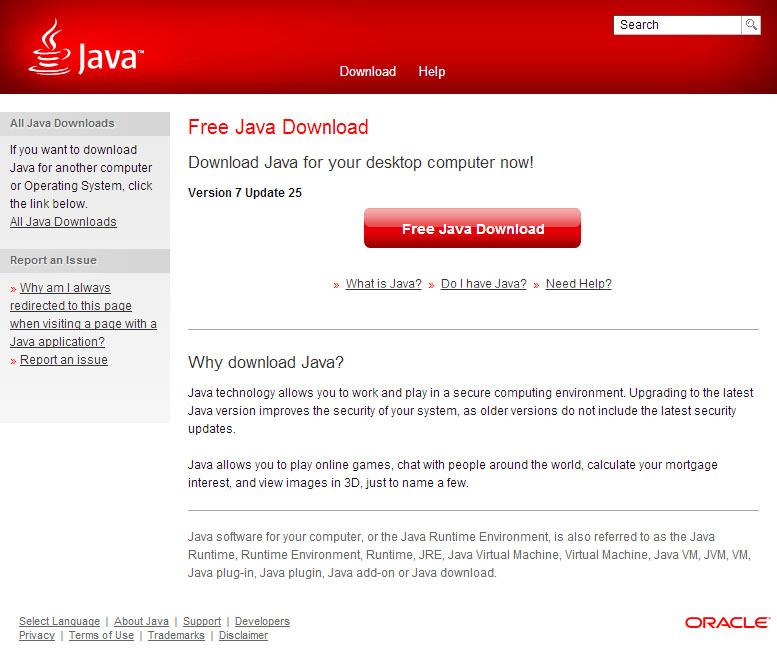
\includegraphics[scale=0.55]{images/javaInstall1.jpg}
	\end{figure}
\pagebreak
  \item Once the download is complete, run the executable file to install Java and follow the on-screen instructions.\footnote{Screenshots are provided for the Windows version of the Java installer.}
	\begin{figure}[!htb]
	\centering
	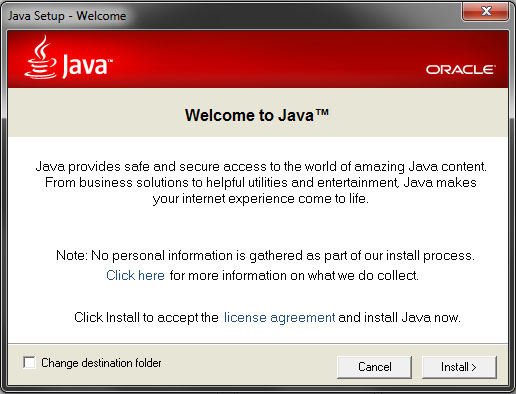
\includegraphics[scale=0.6]{images/javaInstall2.jpg}
	\end{figure}
  \item Once the installation is complete, you will get a pop up message stating that Java has been successfully installed on your computer.
	\begin{figure}[!htb]
	\centering
	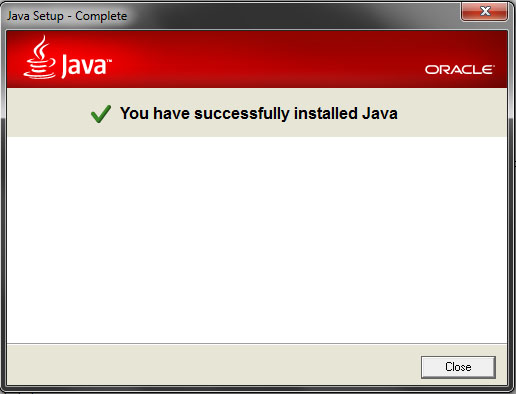
\includegraphics[scale=0.6]{images/javaInstall3.jpg}
	\end{figure}
\end{enumerate}

This is the only installation required in order to run the Vessel Monitoring System correctly.
\clearpage

{\color{royalblue}\subsection{Users Manual}}
\paragraph{Brief Overview \\}

The Vessel Monitoring System(VMS) is a Java-based application that allows its users to check the positions of various types of vessels. This application can only be accessed by current valid users and administrators of the program. To run the program, you will need the two different jar files for the Vessel Monitoring System and the Radar Simulator. The Vessel Monitoring System should be run first, followed by the Radar Simulator once the user has logged into the VMS.

\subsubsection{Vessel Monitoring System}
\paragraph{Login Screen \\}
The Login screen is directly accessed as soon as the VMS program starts. A valid password is required to be allowed to use the program. Only two access levels are available, normal user and administrator. The password for normal user is "user123", and the password for administrator is "op123".

	\begin{figure}[!htb]
	\centering
	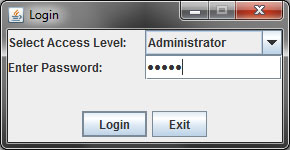
\includegraphics[scale=0.80]{images/userManual1.jpg}
	\end{figure}

\paragraph{Main Screen \\}
After logging in, the Main Screen will appear. This is where all the important information will be displayed. The Main Screen will be different depending on the current user's access level. An administrator will have more options than a normal user. The main screen opens in Table View by default and it consists of:

\subparagraph{1) Menu bar \\}

The menu is where the user can select to logout or exit the program. If the logout option is selected, then the program will return to the Login Screen.
	\begin{figure}[!htb]
	\centering
	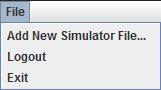
\includegraphics[scale=1]{images/userManual4.jpg}
	\end{figure}

\pagebreak

\subparagraph{2) Table View Tab \\}
In this view, the user can see a list of all the vessels detected by the radar. The color of each row depends on the type of alert the specific vessel is currently involved in. If the user has logged in as an administrator, the vessels can be ordered by any column in ascending or descending order by clicking the header cell at the top of each column in the table.

	\begin{figure}[!htb]
	\caption{Administrator Table View}
	\centering
	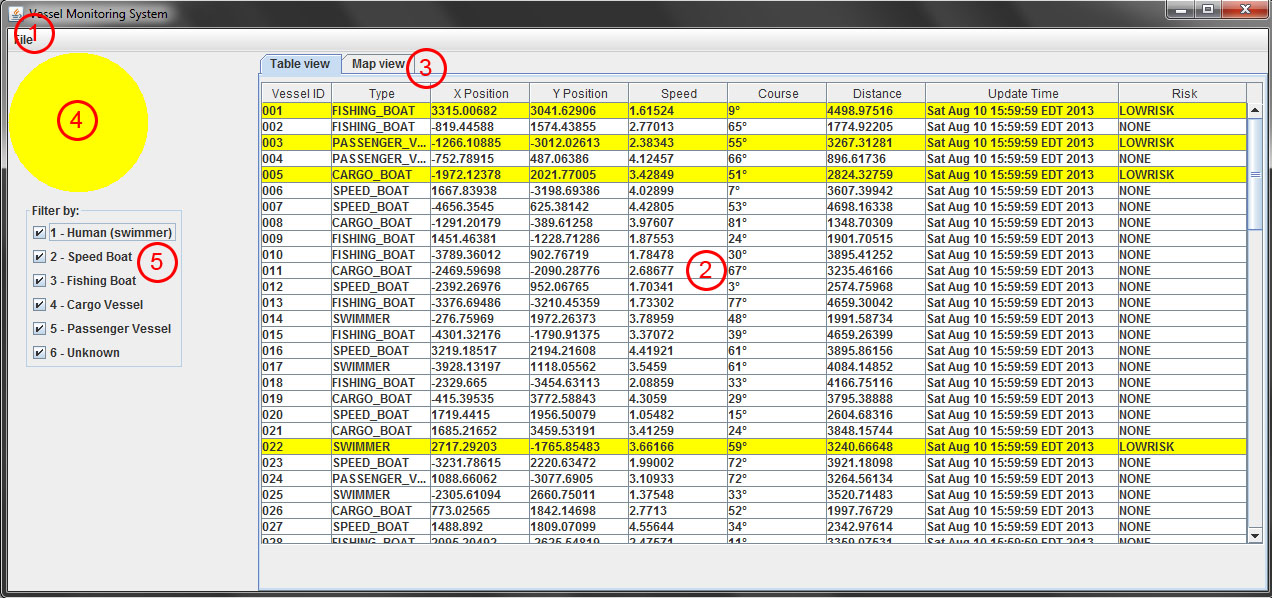
\includegraphics[scale=0.36]{images/userManual2_admin.jpg}
	\end{figure}

	\begin{figure}[!htb]
	\caption{Normal User Table View}
	\centering
	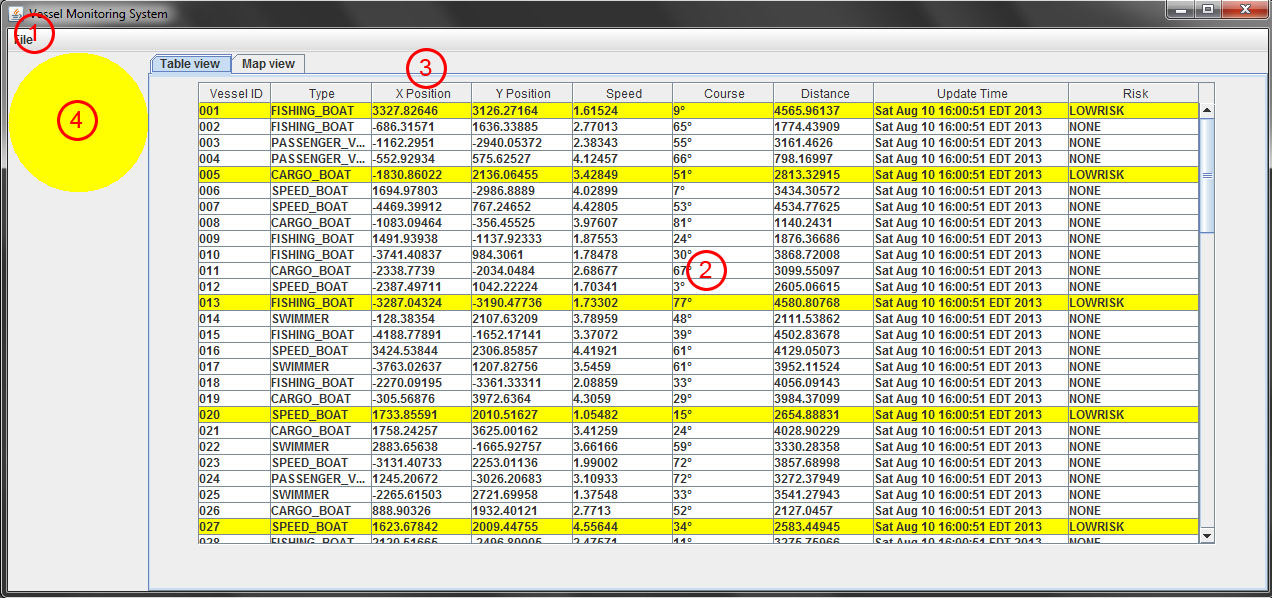
\includegraphics[scale=0.36]{images/userManual2_user.jpg}
	\end{figure}

\break
\subparagraph{3) Map View Tab \\}
In this view, the user can see the vessels displayed on the map. Different types of vessels have different colors. The position of every vessel will be updated over time. The color and visibility of the circles around the vessels will change depending on the alert type of a vessel.
	
	\begin{figure}[!htb]
	\caption{Administrator Map View}
	\centering
	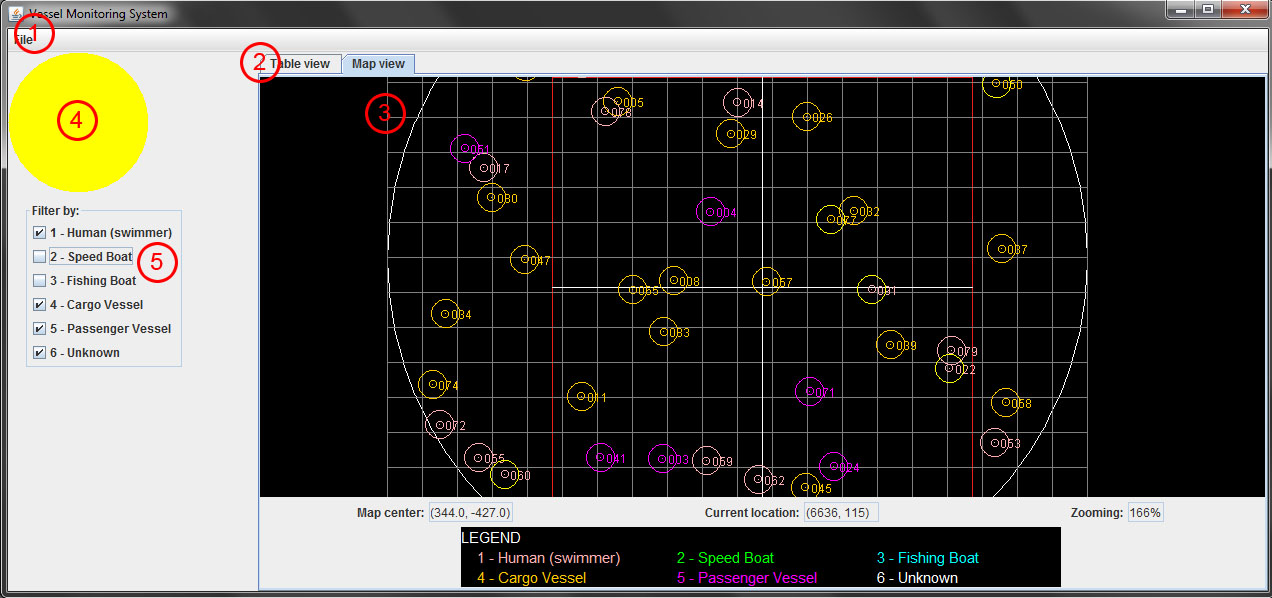
\includegraphics[scale=0.36]{images/userManual3_admin.jpg}
	\end{figure}

	\begin{figure}[!htb]
	\caption{Normal User Map View}
	\centering
	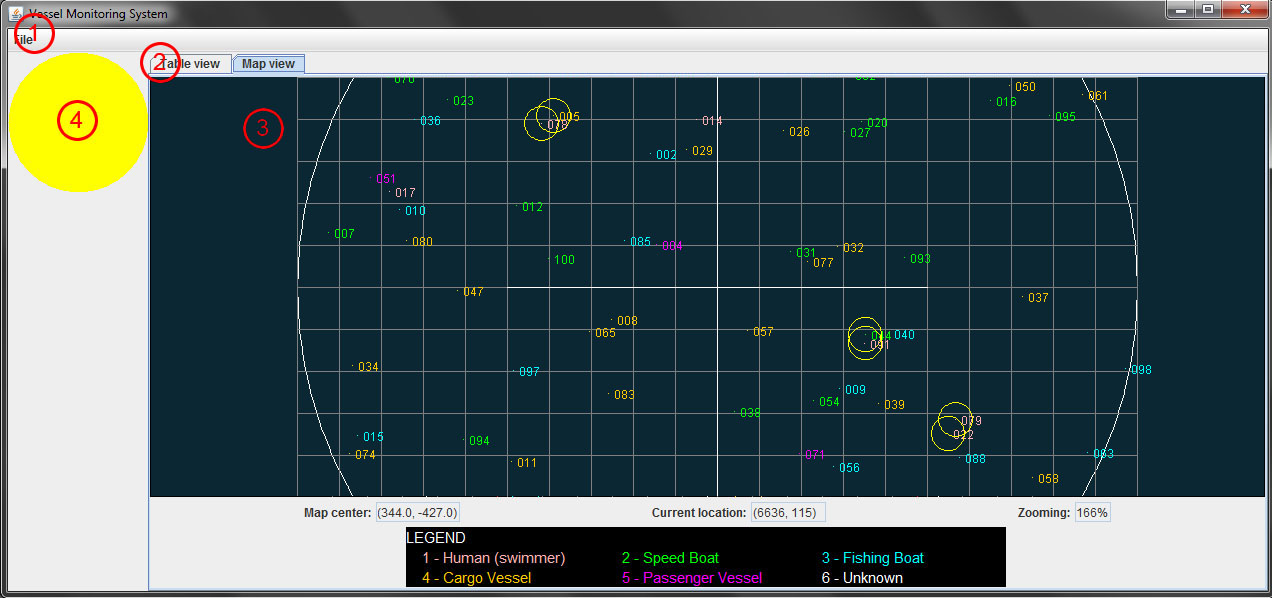
\includegraphics[scale=0.36]{images/userManual3_user.jpg}
	\end{figure}
\break
There is also a zoom functionality in the map tab. It is enabled by scrolling the mouse forward (to zoom in) or backward (to zoom out) on the map area. Zooming is performed on the point of origin. There are two ways to change the point of origin. A user can either click on the map to quickly move the point of origin to the location of the click, or click and drag the map to the desired location. The map will only go within 5000 meters of the default point of origin.\\

\subparagraph{4) Alert Indicator \\}
The alert indicator always displays the color of the current most serious alert. A green circle indicates that all the vessels are a safe distance from one another. A yellow circle indicates that some vessels are very close to one another. A red circle indicates that some vessels are dangerously close to one another and that a collision may occur.\\

\subparagraph{5) Filters \\}
This section is only available if the user has logged in as an administrator. The filters allow the user to hide/show certain types of vessels by deselecting/selecting the proper checkboxes.\\

\subsubsection{Radar Simulator}
The Radar Simulator must be run from the command-line after the user has logged into the Vessel Monitoring System. Using the command prompt, the user should navigate to the folder containing the jar files to run the application. Once in the correct folder, the following line must be written in order to run the Radar Simulator.

\begin{verbatim}
java -jar Simulator.jar --host localhost --port 11233 --input COMP354_50_demo_500.vsf
\end{verbatim}

Here, the host and the port are specific to the machine that is running the Radar Simulator. If both are running on the same machine, then the host should be "localhost" and the port number "11233". The vsf file listed above is an example of a vsf file located in the same folder as the jar files. The user can type the path of any vsf file followed by its complete name to run files in other directories.

\break

{\color{royalbluedark}\section{Final cost estimate}} % Status: Complete

% [This shall consist of a table listing all components of all phases of this project, including the person hours cost of each component of each phase. This should include documentation, design, implementation and testing. Include the meeting minutes with action item and the time log as well]

\begin{figure}[!htb]
\caption{Gantt Chart}
\centering
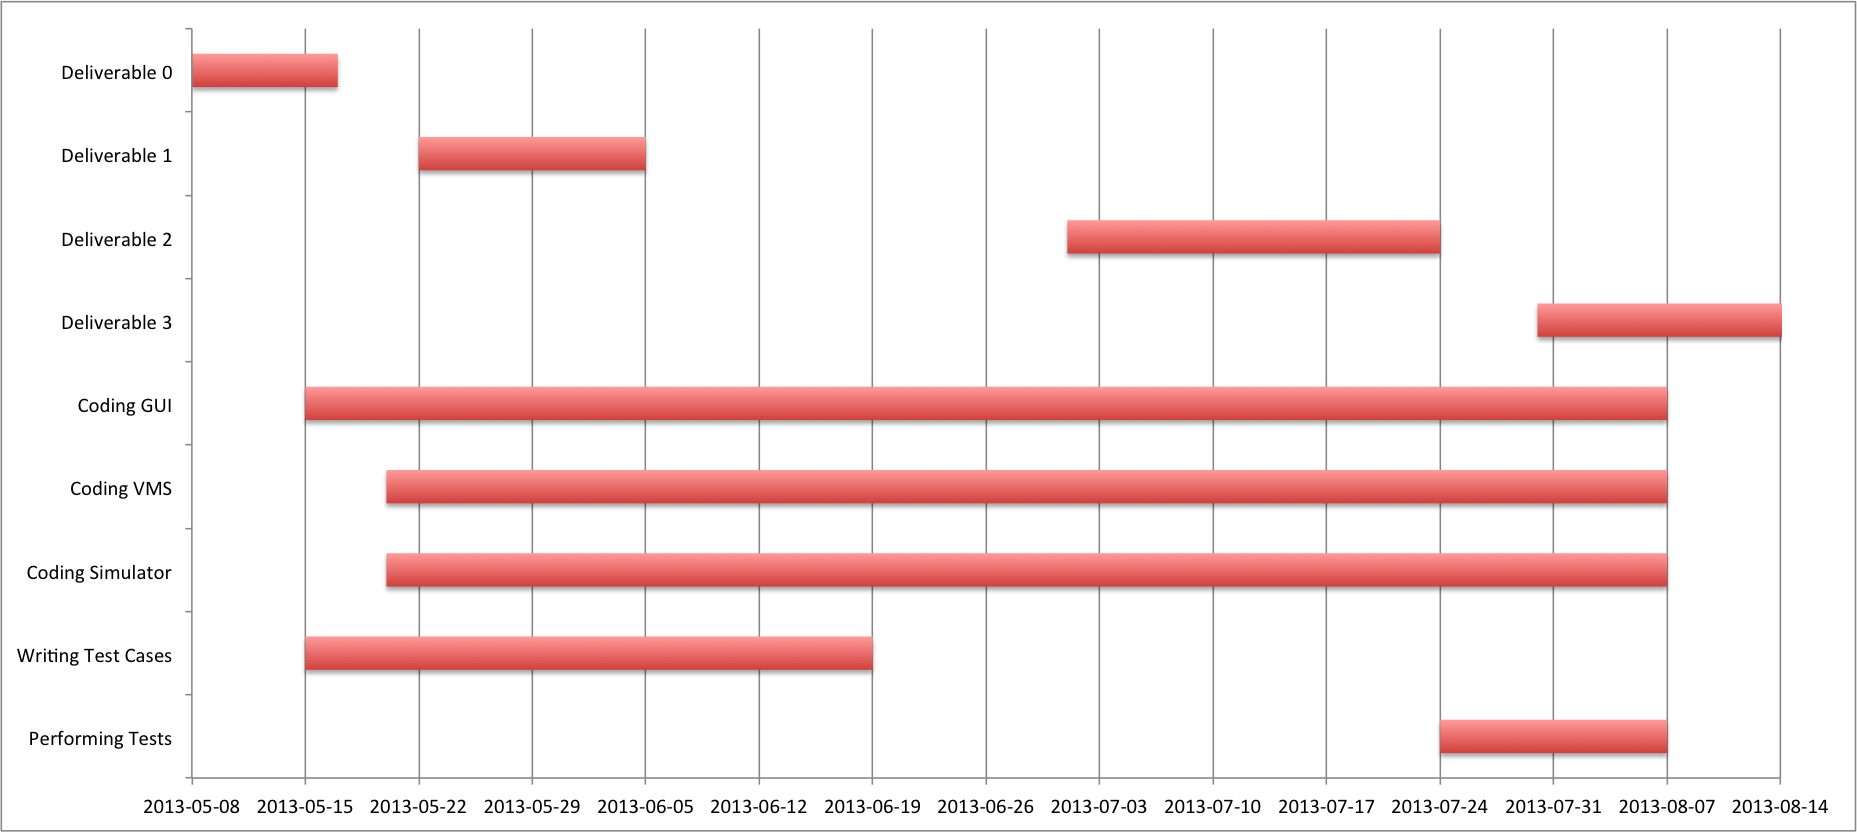
\includegraphics[scale=0.55]{charts/GanttChart.png}
\end{figure}

\begin{table}[ht]
\caption{Final Cost Estimate Table }

\makebox[\textwidth][c]{
\begin{tabular}{|c |c |c |c| }
% centered columns (4 columns)
\hline \hline %inserts double horizontal lines
Components & Estimated Hours  &  Recorded Hours & Associated Cost (\$)\\[0.1ex]
\hline
Deliverable 1 Overview & & &\\
\hline
Role Assignment Meeting  & 1 & 1 & 15\\
Progress Work Report & 2 & 2 & 30\\
Project Description & 3 & 6 & 90\\
Goals and Constraints & 3 & 6 & 90\\
Resource Evaluation & 3 & 6 & 90\\
Scoping and Plan & 	3 & 6 & 90\\
Diagram Description, Domain model, Use Cases & 1 & 2 & 30\\
Coding Phase 1 & 8 & 8 & 120\\
Creating Test Cases & 4 & 5 & 75\\
Project Design & 4 & 5 & 75\\
\hline
Total & 32 & 47 & 705\\[1ex]
\hline
Deliverable 2 Overview & & &\\
\hline		
Role Assignment Meeting & 1 & 1 & 15\\
Architectural Design, Subsystem Interfaces Specifications & 3 & 3 & 45\\
Detailed Design & 3 & 2 & 30\\
Dynamic Design Scenarios & 3 & 2 & 30\\
Program Description, UML Diagram & 6 & 7 & 105\\
Coding Phase 2 & 6 & 6 & 90\\
Creating Test Cases & 2 & 1 & 15\\
Testing & 3 & 2 & 30\\
\hline
Total & 27 & 24 & 360\\
\hline
Deliverable 3 Overview & & &\\
\hline
Role Assignment Meeting & 1 & 2 & 30\\
System Delivery (User Manual, Installation Manual) & 5 & 5 & 75\\
Listing of Tested Items & 5 & 7 & 105\\
Test cases (Units, Requirements) & 10 & 10 & 150\\
Code Completion (Error Fixing \& Recoding) & 5 & 6 & 90\\
Finalizing of Complete Functional Software & 5 & 6 & 90\\
\hline
Total & 31 & 36 & 540\\
\hline
Project Total & 90 & 107 & \$1605\\
\hline
\end{tabular}}
\end{table}

\clearpage

\paragraph{Basis.} Costs have been calculated based on the amount of man hours spent working on project (at a normal approximate labor cost of \$15 an hour). There was no cost associated with tools, because all tools used were either freely available or were provided by the University.

\subsection{Meeting Minutes}

Meeting Minutes can be found in the Meeting Minutes folder

\clearpage

\listoffigures
\clearpage

\end{document}
